\documentclass{article}

\PassOptionsToPackage{numbers, compress}{natbib}
\usepackage[dblblindworkshop]{neurips_2026}
\workshoptitle{AIMO Interpretability Challenge}

\usepackage[utf8]{inputenc}
\usepackage[T1]{fontenc}
\usepackage{hyperref}
\usepackage{url}
\usepackage{booktabs}
\usepackage{amsfonts}
\usepackage{nicefrac}
\usepackage{microtype}
\usepackage{xcolor}
\usepackage{graphicx}

\newcommand{\BBVAL}{0.500}
\newcommand{\BBID}{1021767}

\title{Prompt Probes Read Solve Rate, Not Robustness:\\Negative Results from the AIMO Interpretability Challenge}

\author{Anonymous Author(s)}

\begin{document}

\maketitle

\begin{abstract}
We predict, from one forward pass over the prompt, whether a small reasoning model solves an olympiad problem robustly (Small Models track). A linear probe looked strong on the official training rows (balanced accuracy up to 0.78), but those rows never give different labels to different models on the same problem, so it can succeed by reading problem difficulty. We therefore labeled 102 new problems for three of the four models ourselves. A model's hidden state predicts its own solve rate ($r = 0.70$ to $0.74$), better than the agreement of four sampled answers ($r = 0.56$), but not its robustness: on problems whose labels differ across models no probe clearly beats the per-model majority, and an apparent gain on a larger pool disappeared once problems the organizers flag as leakage-prone were removed. A white-box ablation shows the hidden state carries the signal: replacing it with surface text features halves solve-rate prediction ($r = 0.70$ to $0.33$), and on the official validation set the same head drops from 0.643 to 0.500 without it. A cheap test-time counterfactual check reaches 0.67 to 0.69 on our labels but 0.38 to 0.50 on the organizers'. We document two pitfalls that silently corrupt self-generated labels and release all code and data.
\end{abstract}

\section{Setting}
For a model $m$ and problem $q$, the task is to predict whether $m$'s accuracy on $q$ survives perturbations that keep the deductive chain~\cite{stefanik2026aimointerp}. The Small Models track covers Qwen3.5-4B, Skywork-OR1-Math-7B, Olmo-3-7B-Think and DeepSeek-R1-0528-Qwen3-8B, evaluated offline in 3600\,s on one RTX PRO 6000. Public supervision is 34 labeled rows over 20 problems. Validation and test sets are balanced per problem and per model; always-true scores exactly 0.50 on the 14-case validation set.

\section{A shared prompt probe reads difficulty}
We fit L2 logistic probes on every layer's last-token and mean-pooled prompt states with problem-grouped 5-fold CV (3 seeds). A \emph{shared} probe uses one encoder for all targets plus a target one-hot; a \emph{self} probe uses the target's own states (Figure~\ref{fig:depth}).

\begin{figure}[h]
  \centering
  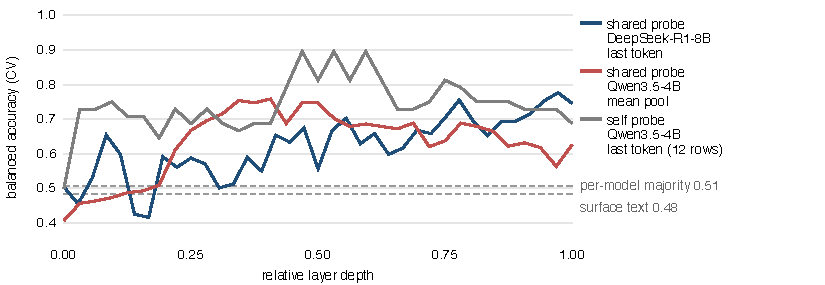
\includegraphics[width=\linewidth]{fig1.pdf}
  \caption{Balanced accuracy on the 34 official rows by relative depth. Surface text features and the per-model majority stay at chance.}
  \label{fig:depth}
\end{figure}

The rising DeepSeek curve (0.72 over the top quarter of layers) is not evidence for the target: of the 9 problems labeled for more than one model, none has differing labels, and the one-hot enters only as a bias, so the probe cannot separate models on one problem. Submitted, it scored 0.643 (9/14).

\section{Self-generated labels}
We sampled 150 integer-answer problems absent from the official data (AIME 2022 to 2026, AMC 12 2022 to 2023, HMMT, BRUMO, SMT, CMIMC) with the organizers' sampling settings ($T = 1.0$, top-$k$ 40, top-$p$ 0.95): 8 samples on the original and, if solved at least once, 6 on each of three rule-based variants (rename, typos, distractor). A problem is robust if the largest family drop is at most 0.10 and spurious if at least 0.25; never-solved problems count as robust. Olmo was dropped (5 concurrent sequences on a 32\,GB GPU). Two pitfalls nearly corrupted the labels. \textbf{Truncation:} at a 12k-token cap 90\% of Qwen3.5-4B samples ended without an answer (mean accuracy 0.10); capping reasoning at 8k and forcing an answer (\texttt{</think> ... \textbackslash boxed\{}) gave 0.49. \textbf{fp8 KV cache:} in vLLM 0.31 Skywork looped on single tokens (accuracy 0.12 on finished answers); bf16 gave 0.98. Following the organizers' advice against validation/test leakage we drop AIME 2024 to 2026 (48 problems). The result is 262 labels on 102 problems; 28 problems (73 rows) have labels that differ across models.

\section{Self-probes: solve rate yes, robustness no}

\begin{table}[h]
  \caption{Out-of-fold balanced accuracy (problem-grouped, 3 seeds); ranges span layer bands and ridge strengths. One standard error on 73 rows is about 6 points.}
  \label{tab:probes}
  \centering
  \small
  \begin{tabular}{lcc}
    \toprule
    Method & mixed problems (73) & official rows (25) \\
    \midrule
    per-model majority & 0.55 & 0.68 \\
    shared probe (Section 2) & 0.58 & 0.59 \\
    self probe, direct, best depth & 0.61 & 0.56 \\
    self probe, solve rate then robustness & 0.47 to 0.51 & 0.35 to 0.51 \\
    self probe, blend of both & 0.47 to 0.54 & 0.45 to 0.61 \\
    sampled base accuracy (reference) & 0.71 & n/a \\
    \bottomrule
  \end{tabular}
\end{table}

A ridge probe on a model's own last-token state predicts its 8-sample solve rate at $r = 0.70$ to $0.74$, whereas the majority agreement of four sampled answers correlates with four other samples' solve rate at only $r = 0.56$. Robustness is another matter: every probe sits within about one standard error of the majority (Table~\ref{tab:probes}). On the full 150-problem pool the blend had looked better (0.63 vs.\ 0.54 majority on 117 rows); dropping the 48 leakage-prone problems took it to 0.53, a reminder of how optimistic small mixed subsets are. Drawing one robust and one spurious model per mixed problem (Figure~\ref{fig:draws}), knowing which model is more often robust gives 0.63, ranking by raw probe score gives no more (0.50 to 0.59), and scores standardized per model or thresholded at each model's median fall to 0.37 to 0.51.

\begin{figure}[h]
  \centering
  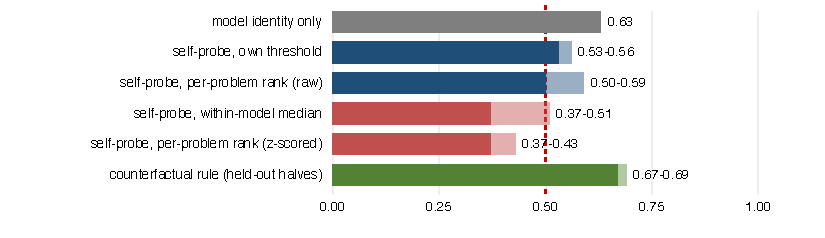
\includegraphics[width=\linewidth]{fig2.pdf}
  \caption{Accuracy on per-problem balanced draws of our labels (chance dashed; ranges over seeds). Red rules remove model identity.}
  \label{fig:draws}
\end{figure}

\paragraph{White-box ablation.} We remove the hidden state and keep everything else. On our labels we rerun the same per-model probe (last token, relative depth 0.6 to 0.8, same rows and folds) with black-box inputs: four surface text features of the problem (length, digit count, LaTeX density, largest number) plus the target one-hot. On the official validation set we refit the submitted blend head on the same training pool with the same recipe, replacing the hidden state by the same four text features, and submit it under the identical Small-track protocol (Codabench submission \BBID); for Olmo, where the self-probe falls back to a shared hidden-state probe, the black-box entry predicts the constant fallback.

\begin{table}[h]
  \caption{White-box ablation. Robustness columns are balanced accuracy on our held-out labels (out-of-fold) and accuracy on the 14-case Codabench validation set (Small Models track); solve rate is out-of-fold Pearson $r$.}
  \label{tab:ablation}
  \centering
  \small
  \begin{tabular}{lcccc}
    \toprule
    Inputs & solve rate $r$ & mixed (73) & official (25) & validation (14) \\
    \midrule
    own hidden state (white-box) & 0.70 & 0.57 & 0.65 & 0.643 \\
    text features + model one-hot & 0.33 & 0.45 & 0.49 & \BBVAL \\
    per-model majority / always-true & n/a & 0.55 & 0.68 & 0.500 \\
    \bottomrule
  \end{tabular}
\end{table}

Removing the hidden state halves solve-rate prediction and costs about 12 points of robustness accuracy on mixed problems, so the internal signal is what carries the probe; the white-box probe still does not clearly beat the per-model majority on robustness. On the validation set the same blend head drops from 0.643 (9/14) to 0.500 (7/14) without the hidden state; 2 cases out of 14 is within noise but points the same way.

Our submitted self-probe (trained on all 150 problems) scored 0.643 (9/14) on Codabench, the same as the shared probe. A version retrained without AIME 2024 to 2026 (\texttt{submissions/self-probe-v2}) scored 0.571 (8/14) and is nominated alongside it.

\section{A test-time counterfactual check does not transfer}
We then measured behaviour at test time: the target answers the original twice and each variant once under a time-managed budget (8k down to 1k tokens), and a problem is robust if no variant loses more than 0.1 of the model's own majority answer.

\begin{table}[h]
  \caption{The same rule against our labels and the organizers' labels.}
  \label{tab:cf}
  \centering
  \small
  \begin{tabular}{lcc}
    \toprule
    Evaluation & counterfactual & reference \\
    \midrule
    our labels, balanced (held-out halves) & 0.67 to 0.69 & self probe 0.37 to 0.51 \\
    34 official rows (RTX 5090, 3072\,s) & 0.38 (bal.\ 0.48) & always-true 0.68 \\
    Codabench validation (14) & 0.50 & self probe 0.643 \\
    \bottomrule
  \end{tabular}
\end{table}

It predicts only 9 of 34 official rows robust (70\% are). Five samples let one unstable answer flip the call, while the official labels use more samples, budgets up to 100k tokens and LLM-written perturbations; agreement with our labels came from sharing our choices.

\section{Discussion}
Prompt representations encode whether a model can solve a problem, not whether its solution survives perturbation. Validating probes only on rows without per-problem label variation, or without a model-identity baseline, hides this, and self-generated labels inherit their generator's budget, perturbations and sample counts. The final entry (\texttt{submissions/self-probe}) runs the 34 official rows offline in 38\,s. Labels, generations and all scripts are in the supplementary material (about USD 10 of rented GPU time in total) and will be released as a public repository after review.

\section*{Limitations}
The study covers 102 problems, three of the four track models, an 8k reasoning budget, rule-based perturbations and the never-solved-is-robust convention; the Codabench validation set has only 14 cases, so one case moves accuracy by 7 points.

\section*{AI Use Statement}
In this work, we used generative AI tools (Anthropic Claude, through an agentic assistant) for ideation (experiment design and literature search), coding (label generation, probe training and analysis scripts), analysis (interpreting results and making figures) and writing (drafting and editing this report). We did not use generative AI tools to produce the labels or model outputs studied here; these come from the target models themselves, and the research direction and the final choices of claims and submissions were made by the authors. We have reviewed all AI-assisted work and take responsibility for the final content of this paper.

\begin{thebibliography}{1}
\bibitem{stefanik2026aimointerp}
Michal {\v{S}}tef{\'{a}}nik, Philipp Mondorf, Andreas Waldis, Qianying Liu, Chuan Yang, Michal Spiegel, Josef Kucha{\v{r}}, Marek Kadl{\v{c}}{\'{\i}}k, Adam Vawda{-}Oomerjee, Chaoran Liu, Simon Frieder, Barbara Plank, Fazl Barez, and Pontus Stenetorp.
\newblock {AIMO} Interpretability Challenge.
\newblock \emph{CoRR}, abs/2607.13899, 2026.
\newblock \url{https://doi.org/10.48550/arXiv.2607.13899}.
\end{thebibliography}

\end{document}
